\documentclass[10pt]{article}
\usepackage{graphicx}
\usepackage{hyperref}
\usepackage{amsmath}
\usepackage{enumitem}
\usepackage{cite}
\usepackage[labelfont=bf]{caption}
\usepackage{float}
\usepackage{listings}
\usepackage{lstautogobble}
\usepackage{adjustbox}
\usepackage{tabularx}
\usepackage{indentfirst}

%\emergencystretch=1em

\lstset{basicstyle=\ttfamily,
  mathescape=true,
  escapeinside=||,
  autogobble}

% Copyright 2017 Sergei Tikhomirov, MIT License
% https://github.com/s-tikhomirov/solidity-latex-highlighting/

\usepackage{listings, xcolor}

\definecolor{verylightgray}{rgb}{.97,.97,.97}

\lstdefinelanguage{Solidity}{
	keywords=[1]{anonymous, assembly, assert, balance, break, call, callcode, case, catch, class, constant, continue, contract, debugger, default, delegatecall, delete, do, else, emit, event, export, external, false, finally, for, function, gas, if, implements, import, in, indexed, instanceof, interface, internal, is, length, library, log0, log1, log2, log3, log4, memory, modifier, new, payable, pragma, private, protected, public, pure, push, require, return, returns, revert, selfdestruct, send, storage, struct, suicide, super, switch, then, this, throw, transfer, true, try, typeof, using, value, view, while, with, addmod, ecrecover, keccak256, mulmod, ripemd160, sha256, sha3}, % generic keywords including crypto operations
	keywordstyle=[1]\color{blue}\bfseries,
	keywords=[2]{address, bool, byte, bytes, bytes1, bytes2, bytes3, bytes4, bytes5, bytes6, bytes7, bytes8, bytes9, bytes10, bytes11, bytes12, bytes13, bytes14, bytes15, bytes16, bytes17, bytes18, bytes19, bytes20, bytes21, bytes22, bytes23, bytes24, bytes25, bytes26, bytes27, bytes28, bytes29, bytes30, bytes31, bytes32, enum, int, int8, int16, int24, int32, int40, int48, int56, int64, int72, int80, int88, int96, int104, int112, int120, int128, int136, int144, int152, int160, int168, int176, int184, int192, int200, int208, int216, int224, int232, int240, int248, int256, mapping, string, uint, uint8, uint16, uint24, uint32, uint40, uint48, uint56, uint64, uint72, uint80, uint88, uint96, uint104, uint112, uint120, uint128, uint136, uint144, uint152, uint160, uint168, uint176, uint184, uint192, uint200, uint208, uint216, uint224, uint232, uint240, uint248, uint256, var, void, ether, finney, szabo, wei, days, hours, minutes, seconds, weeks, years},	% types; money and time units
	keywordstyle=[2]\color{teal}\bfseries,
	keywords=[3]{block, blockhash, coinbase, difficulty, gaslimit, number, timestamp, msg, data, gas, sender, sig, value, now, tx, gasprice, origin},	% environment variables
	keywordstyle=[3]\color{violet}\bfseries,
	identifierstyle=\color{black},
	sensitive=false,
	comment=[l]{//},
	morecomment=[s]{/*}{*/},
	commentstyle=\color{gray}\ttfamily,
	stringstyle=\color{red}\ttfamily,
	morestring=[b]',
	morestring=[b]"
}

\lstset{
	language=Solidity,
	backgroundcolor=\color{verylightgray},
	extendedchars=true,
	basicstyle=\footnotesize\ttfamily,
	showstringspaces=false,
	showspaces=false,
	%numbers=left,
	%numberstyle=\footnotesize,
	%numbersep=9pt,
	tabsize=2,
	breaklines=true,
	showtabs=false,
	captionpos=b
}

% wide margins
\addtolength{\oddsidemargin}{-.75in}
\addtolength{\evensidemargin}{-.75in}
\addtolength{\textwidth}{1.5in}
\addtolength{\topmargin}{-.875in}
\addtolength{\textheight}{1.75in}
% \captionsetup[table]{skip=4pt}

%%%%%%%%%%%%%%%%%%%%%%%%%%%%%%%%%%%%%%%%%%%%%%%%%%%%%%%%%%%%%%%%%%%%%%%%%%%%%%%%
%~~~~~~~~~~~~~~~~~~~~~~~~~~~~~~~~~~~~~~~~~~~~~~~~~~~~~~~~~~~~~~~~~~~~~~~~~~~~~~%
%%%%%%%%%%%%%%%%%%%%%%%%%%%%%%%%%%%%%%%%%%%%%%%%%%%%%%%%%%%%%%%%%%%%%%%%%%%%%%%%

% STARTING DOCUMENT
\begin{document}

%%%%%%%%%%%%%%%%%%%%%%%%%%%%%%%%%%%%%%%%%%%%%%%%%%%%%%%%%%%%%%%%%%%%%%%%%%%%%%%%
%~~~~~~~~~~~~~~~~~~~~~~~~~~~~~~~~~~~~~~~~~~~~~~~~~~~~~~~~~~~~~~~~~~~~~~~~~~~~~~%
%%%%%%%%%%%%%%%%%%%%%%%%%%%%%%%%%%%%%%%%%%%%%%%%%%%%%%%%%%%%%%%%%%%%%%%%%%%%%%%%

% START TITLE PAGE
\title{\textbf{Kosu: A Decentralized Relay Protocol for Smart Contract Based Financial Primitives}} 
\author{Liam Kovatch, Henry Harder \\\texttt{www.kosu.io}}
\date{\today}
\maketitle
% END TITLE PAGE

%%%%%%%%%%%%%%%%%%%%%%%%%%%%%%%%%%%%%%%%%%%%%%%%%%%%%%%%%%%%%%%%%%%%%%%%%%%%%%%%
%~~~~~~~~~~~~~~~~~~~~~~~~~~~~~~~~~~~~~~~~~~~~~~~~~~~~~~~~~~~~~~~~~~~~~~~~~~~~~~%
%%%%%%%%%%%%%%%%%%%%%%%%%%%%%%%%%%%%%%%%%%%%%%%%%%%%%%%%%%%%%%%%%%%%%%%%%%%%%%%%

%BEGIN ABSTRACT
\begin{abstract}
   We motivate Kosu: a decentralized network and protocol that encourages the curation of a consistent, high-quality, and verifiable public order book. The Kosu network is an independent bonded proof-of-stake blockchain built on Tendermint Consensus. The lightweight state application is responsible for enforcing a simple access control rule-set and order booking procedure. The network utilizes a shared security model, wherein all staking and token-based mechanics happen on the Ethereum main-network. The model provides unidirectional communication and checkpoints between the two networks by leveraging Tendermint to provide finality for specific Ethereum-based state changes. Individuals intending to post orders to the Kosu network are required to bond tokens for the duration they wish to have access. The poster bonding mechanism creates a market for the allocation of network resources throughput and an implicit incentive to contribute quality liquidity to the network. Kosu validators are selected via a token curated registry system on Ethereum. This registry system allows both the inflation rate as well as the number of active validators to be market driven and determined by the network’s stakeholders. The network is highly generalizable, supporting orders of arbitrary maker-taker based virtual settlement systems. In its entirety, the proposed system effectively curates a decentralized order book that serves as a liquidity aggregation primitive for second layer systems. Kosu will be free to use and open source, reducing barriers to entry for both developers and market agents. // TODO: review and finalize
   \medskip
\end{abstract}
\pagebreak
% END ABSTRACT

%%%%%%%%%%%%%%%%%%%%%%%%%%%%%%%%%%%%%%%%%%%%%%%%%%%%%%%%%%%%%%%%%%%%%%%%%%%%%%%%
%~~~~~~~~~~~~~~~~~~~~~~~~~~~~~~~~~~~~~~~~~~~~~~~~~~~~~~~~~~~~~~~~~~~~~~~~~~~~~~%
%%%%%%%%%%%%%%%%%%%%%%%%%%%%%%%%%%%%%%%%%%%%%%%%%%%%%%%%%%%%%%%%%%%%%%%%%%%%%%%%

% TABLE OF CONTENTS
\tableofcontents
\pagebreak
% END TABLE OF CONTENTS

%%%%%%%%%%%%%%%%%%%%%%%%%%%%%%%%%%%%%%%%%%%%%%%%%%%%%%%%%%%%%%%%%%%%%%%%%%%%%%%%
%~~~~~~~~~~~~~~~~~~~~~~~~~~~~~~~~~~~~~~~~~~~~~~~~~~~~~~~~~~~~~~~~~~~~~~~~~~~~~~%
%%%%%%%%%%%%%%%%%%%%%%%%%%%%%%%%%%%%%%%%%%%%%%%%%%%%%%%%%%%%%%%%%%%%%%%%%%%%%%%%

% BEGIN INTRO
\section{Introduction}\label{intro}
Historically, financial markets have been relatively siloed. To date, centralized entities control significant entry points and accounting systems, limiting access beyond a small set of privileged participants. The recent invention of blockchains, decentralized ledger systems, is now challenging this trusted paradigm. Ethereum, a public blockchain with a built-in Turing-complete programming language, provides developers an immutable and verifiable computation platform for scripts known as “smart-contracts”. These scripts can encode arbitrary, deterministic state transition functions, providing a powerful primitive for more complex ledger based application systems.
\medskip

Since the network’s genesis in 2014, developers have leveraged smart contracts for a wide range of novel protocol systems. Perhaps the most adopted technical standard for smart contracts is the ERC-20 token implementation. The standard defines a common token interface allowing for the creation of a diverse set of Ethereum-based assets. These tokens often serve as a critical crypto economic primitive providing core utility for protocol systems also deployed on Ethereum. As such, a system of exchange is a key requisite in a mature token-dependent contract ecosystem.
\medskip

In early 2017, the 0x Project published a whitepaper defining a maker-taker based exchange  protocol in which a pipeline of publicly accessible Ethereum smart contracts facilitate the wallet-to-wallet settlement of funds. In this model, order broadcast and discovery happen off-chain. Independent entities known as relayers are responsible for sourcing and maintaining liquidity in the form of independent collections of signed order messages. This hybrid architecture drastically improved the efficiency of existing DEX systems while also providing a critical open exchange primitive with high extensibility. Since the first deployment of the 0x protocol, a significant number have adopted it as a common piece of infrastructure. To date, the team continues to push the limits on scalability, efficiency and incentivization for DEX systems.
\medskip

Virtual settlement systems, specifically decentralized exchanges (DEXs), are a relatively accessible use case for blockchains; a direct evolution from the original digital currency use-case. While conceptually apparent, the architecture of DEXs is a complex and evolving subject. The scalability restraints of blockchain systems combined with the complexities of an asynchronous discrete time system limit their compatibility with optimally efficient continuous time order books and settlement systems. As such, alternative DEX architectures have also captured considerable market share. These systems include dutch auctions and automated market making systems. While immediately compelling for some use cases, the evolution towards hybrid continuous time order books is likely inevitable. These systems, though currently constrained, likely represent the most scalable and efficient DEX structure.
\medskip

The Kosu network is designed within the 0x-motivated ecosystem, providing a decentralized aggregation primitive for arbitrary limit orders. More specifically, the Kosu network aims to provide a highly extensible decentralized complement to independent centralized aggregators, or relayers. The set of orders maintained on the Kosu network should represent a high-value subset of the compatible order universe.

\clearpage
\pagebreak
% END INTRO

%%%%%%%%%%%%%%%%%%%%%%%%%%%%%%%%%%%%%%%%%%%%%%%%%%%%%%%%%%%%%%%%%%%%%%%%%%%%%%%%
%~~~~~~~~~~~~~~~~~~~~~~~~~~~~~~~~~~~~~~~~~~~~~~~~~~~~~~~~~~~~~~~~~~~~~~~~~~~~~~%
%%%%%%%%%%%%%%%%%%%%%%%%%%%%%%%%%%%%%%%%%%%%%%%%%%%%%%%%%%%%%%%%%%%%%%%%%%%%%%%%

% BEGIN OVERVIEW SECTION
\section{Overview}\label{overview}

Kosu is chiefly composed of two interdependent systems that together implement the protocol’s core functionality of order message relay and the establishment of a consistent set of recent orders. The Kosu contract system supports the protocol's incentive mechanisms, validator curation by stakeholders, and sybil tolerance for the Kosu network, which supports base-layer order book functionality for exchange and liquidity systems built atop it.\footnote{See section \ref{specification} for details on each of these systems.}
\medskip

The first system is the Kosu blockchain, a collection of globally distributed nodes that collectively maintain and update the network’s shared state and "order book"\footnote{The Kosu order book is a set of hashes of specific recent orders, from which conventional limit order books can be constructed. See section TODO}, and maintain a one-way Peg with the Ethereum blockchain. The network supports basic order booking functionality, access control for user accounts, and cryptographic proofs of the existence of state contents, including the set of orders comprising the "order book". Validators secure the network by voting on state changes to an Ethereum contract system, processing orders, and reaching consensus with other validators\footnote{Kosu non-validating full nodes crucially provide access to the order book and enable users to submit orders, laying the foundation for a wide array of applications. Full nodes also allow a wide variety of proofs to be constructed about the existence or absence of state data.} on the canonical chain and the overall application state. In short, Kosu is a bonded proof-of-stake blockchain secured by Tendermint Consensus\cite{tendermint}.
\medskip

The second and closely related component is the Kosu protocol smart-contract system. These contracts are deployed to Ethereum and implement Kosu’s native token and incentive mechanisms, support access control and sybil tolerance for posters, and allow stakeholders to curate the Kosu network’s validator set through a novel token-weighted voting system.
\medskip

Kosu validators run full Ethereum nodes and are responsible for submitting special attestation transactions to the Kosu network about specific state changes to the protocol’s contract system. The only contract state changes the network must reflect are updates to users bonded token balances (which affect a order rate limit enforced by the network), and updates to a dynamic registry contract containing the list of validators stakeholders have currently approved. 
\medskip

Posters who wish to leverage the network’s decentralized order booking and message relay features can gain write access to the network by bonding any amount of Kosu tokens in a specific contract. After their bond transaction is confirmed on Ethereum to a certain depth, validators update the Kosu network's shared state to reflect the bonded balance change of the new poster. The same mechanism allows posters to adjust the amount of tokens they have bonded, or withdraw entirely from the system at any time.
\medskip

At deterministic intervals based on the height of the Ethereum blockchain, Kosu validators compute a simple rate-limit mapping based on in-state balance data that allocates network throughput proportionally to posters who have Kosu tokens bonded at the height a new interval starts. These intervals are called rebalance periods and allow the relatively continuous process of balance updates on the Ethereum Poster Registry as a result of bonding/unbonding by posters to be mapped to more discrete periods of bandwidth limiting in a deterministic manner. At the beginning of each new rebalance period, validators must reach consensus on the parameterization of the upcoming period. The starting and ending Ethereum block heights of the period, and the total number of orders to be accepted from posters during that time is determined prior to allowing posters write access for the period.
\medskip

During normal network operations between rebalance periods, validators accept and process incoming order transactions from posters that have been gossiped to them through full nodes, while submitting regular attestations (called witness transactions) to other validators on the network to ensure the state of the Kosu Ethereum contract system is accurately tracked.
\medskip

The validity of order transactions is based solely on the signature of the poster that submitted the order to the network, and a certain required data structure that enables recovery of the signature. If a valid poster signature is included in the incoming Order and the recovered address matches that of a poster account with a non-zero remaining limit for the current rebalance period, validators will accept the order and include it in a block and decrement the posters bandwidth allocation limit for that period. Otherwise, the order is rejected.
\medskip

The Kosu network uses a bonded proof-of-stake security model wherein validators stake (by locking) tokens into a contract proportional to the amount of vote power they wish to receive. The number of tokens they associate with their stake are locked for the duration the entity wishes to validate. The validator may be stripped of their power at any time at the discretion of voting token holders, and if voted out, their tokens are distributed to the individuals responsible for raising – and voting in – the successful challenge. 
\medskip

During the continuous validator governance and curation process, individuals wishing to become validators submit proposals in which they specify a positive or negative reward schedule. If this value is positive, the validator will be rewarded newly minted tokens that inflate the existing supply. If the value is negative, validators will be required to constantly collateralize their listing at the rate specified so their tokens may be burned. In this case, the negative "reward" deflates the existing supply. 
\medskip

The ability for validators to specify both negative and positive reward rates is a crucial component of the overall system design. For the nascent network, validators will be able to extract little value from the act of validating alone, thus will require inflationary rewards that justify the costs of managing validator infrastructure. However, in a mature state the Kosu network could present incredible value to validators in the form of an informational advantage with regards to who sees new orders first.
\medskip

Validators see proposed and newly committed blocks prior to the rest of the network, and at scale, this information can be monetized. In order for the incentives to remain properly aligned in these conditions, the same aspect of the protocol's design that enables the inflationary reward mechanism, also enables validators to compete by essentially offering to pay for a validating position. The "payment" comes in the form of removing tokens from circulation (burning), which increases the value of all remaining tokens due to the decrease in supply, assuming no or little change in demand.

\clearpage
\pagebreak
% END OVERVIEW SECTION

%%%%%%%%%%%%%%%%%%%%%%%%%%%%%%%%%%%%%%%%%%%%%%%%%%%%%%%%%%%%%%%%%%%%%%%%%%%%%%%%
%~~~~~~~~~~~~~~~~~~~~~~~~~~~~~~~~~~~~~~~~~~~~~~~~~~~~~~~~~~~~~~~~~~~~~~~~~~~~~~%
%%%%%%%%%%%%%%%%%%%%%%%%%%%%%%%%%%%%%%%%%%%%%%%%%%%%%%%%%%%%%%%%%%%%%%%%%%%%%%%%

% BEGIN TECH SPEC SECTION
\section{Specification}\label{specification}

The specification for each of the systems in this section serves communicate the purpose and functionality of each component, rather than provide a fully accurate description of each implementation detail. Thus, most nuanced components are referenced at a high level of abstraction for the sake of brevity and digestibility. Each component of the protocols implementation is open source\cite{paradigm-github} and should be referred to for detailed and up-to-date specification and implementation. 

%%%%%%%%%%%%%%%%%%%%%%%%%%%%%%%%%%%%%%%%%%%%%%%%%%%%%%%%%%%%%%%%%%%%%%%%%%%%%%%%
% BEGIN ORDER SPECIFICATION SUB-SECTION
\subsection{Orders}\label{orders}

The Kosu protocol defines a simple and extensible data structure to represent signed order messages on the network. The primary purpose of the defined order schematic is to allow signature recovery for the verification of poster bandwidth allocations, during the network’s order verification process.
\medskip

The order format described below is also designed to allow the “wrapping” of already existing hybrid-decentralized order message formats (such as 0x and Dharma) for relay on the Kosu network, and settlement through a system of generalizable forwarding contracts. 
\medskip 

Usage of the forwarding contract system is strictly optional, and unrelated to the core protocol in the sense that no state is shared between the protocol contract system, and settlement contracts.

\subsubsection{SubContract interface}\label{subcontract-interface}

Kosu can act as an order message aggregator and/or transport layer for a variety of types of on-chain exchange systems. To achieve this, a simple and extensible contract-based interface is defined that allows a common order message format to be used for a variety of Ethereum settlement pipelines that leverage hybrid decentralized exchange architecture. // link to definition of this term
\medskip

All current SubContract implementations are in Solidity and designed for use with Ethereum, however, any language and blockchain that supports contract-like settlement implementations that satisfy the interface above, and the correct signature scheme, can be used with Kosu.
\medskip

% Begin table 1
\bgroup
\def\arraystretch{1.2}
\begin{table}[H]
\centering
\label{table:table1}
\begin{tabularx}{1\textwidth}{|l|l|X|p{8cm}|}
\hline
\textbf{Method name} & \textbf{Returns} & \textbf{Params.} & \textbf{Description} \\ 
\hline
\texttt{makerArguments} & \texttt{string} & \texttt{-} & Returns a JSON string containing a data structure that specifies the required fields for maker orders for the SubContract. \\
\hline
\texttt{takerArguments} & \texttt{string} & \texttt{-} & Returns a JSON string containing a data structure (identical to \texttt{makerArguments}) that specifies the values a taker must supply when filling a maker order. \\
\hline
\texttt{isValid} & \texttt{boolean} & \texttt{makerData} & Checks weather a maker order is valid and fillable based on the SubContract's validation implementation \\
\hline
\texttt{amountRemaining} & \texttt{uint256} & \texttt{makerData} & For settlement types that support it, this method can return information that allows partial fills \\
\hline
\texttt{participate} & \texttt{boolean} & \texttt{makerData}, \texttt{takerData} & The main settlement logic implementation for SubContracts, which triggers execution of a trade by the taker submitting the maker data and their counter-party information. \\
\hline
\end{tabularx}
\caption{Describes the SubContract interface and method signatures in a language-independent manner.} 
\end{table}
\egroup
% End table 1

Some of the data structures used by the \texttt{SubContract} interface and Kosu order message structure are described in more detail below. The full interface definition in Solidity can be found on the \texttt{ParadigmFoundation} GitHub\cite{kosu-sdk}.

\begin{itemize}
  \item \texttt{makerArguments}: a structure that defines the name and types of each argument in the \texttt{makerValues}
  \item \texttt{takerArguments}: defines the arguments (name and type) takers must provide to \texttt{participate} 
  \item \texttt{makerData}: an array of 32 byte slices of serialized data included in the maker order
  \item \texttt{takerData}: an array of 32 byte slices of serialized data provided by the taker as arguments
\end{itemize}

Since validity conditions of a given order vary greatly between settlement systems, a generic validation interface method (\texttt{isValid}) is provided. A method that returns an arbitrary integer (\texttt{amountRemaining}) is also specified, which can be used to support partial fills for settlement types where it is logical, such as spot exchange implementations.

\subsubsection{Order message format}\label{order-message-format}

A simple order message format is defined based on the SubContract interface. The data structure was specifically designed to satisfy the following requirements:

\begin{enumerate}
  \item Compatibility existing hybrid off-chain settlement systems (0x\cite{0x-wp}, Dharma\cite{dharma-wp}, etc.)
  \item Representable as human-readable, language independent message format (JSON)
  \item Efficient serialization and lossless compression with existing transport layers in mind
  \item Support serialization to Solidity (and Ethereum) compatible data types and structures
  \item Support for arbitrary signature schemes, and a special required signature from a poster\footnote{Described in more detail in the contracts and network sections, a "poster" is any entity that has bonded Kosu tokens in the Poster Registry contract. Doing so affords rate-limited write-access to the Kosu "order book" proportional to stake size.}
\end{enumerate}

The Kosu order message format is described below in a language-independent manner, however the type annotations indicate the JSON type each top-level field is serialized to. The underlying structure of the non-primitive types (\texttt{array} and \texttt{object}) can in the protocols implementation\cite{kosu-monorepo} and documentation.

% Begin table 2
\bgroup
\def\arraystretch{1.2}
\begin{table}[H]
\centering
\label{table:table2}
\begin{tabularx}{1\textwidth}{|l|l|l|X|}
\hline
\textbf{Field name} & \textbf{Type} & \textbf{Required} & \textbf{Description} \\
\hline
\texttt{subContract} & \texttt{string} & yes & The deployed address of the target SubContract settlement implementation. Defines expected arguments. \\
\hline
\texttt{maker} & \texttt{string} & yes & The address of the party that signed the maker order. Usually indicates the beneficiary of settled funds. \\
\hline
\texttt{makerArguments} & \texttt{array} & no & An array of equal length to the number of \texttt{makerArguments} containing objects that define the name and data-type for each argument. \\
\hline
\texttt{takerArguments} & \texttt{array} & no & Similar to \texttt{makerArguments}, it defines the values and data-types required for settlement. Not required for maker orders. \\
\hline
\texttt{makerValues} & \texttt{object} & yes & A hash-map data structure that contains the parameters necessary for a valid maker order of the target settlement type. \\
\hline
\texttt{makerSignature} & \texttt{object} & no & An optional field that can be used to include a signature from the maker. May also be included in \texttt{makerValues}. \\
\hline
\texttt{posterSignature} & \texttt{object} & yes & Stores the signature resulting from a poster entity signing a hash of the maker order values. Used to verify poster has bonded tokens. \\
\hline
\end{tabularx}
\caption{Generic and high-level description of the Kosu Order message format, including optional fields.} 
\end{table}
\egroup
% End table 2
% END ORDERS SUB-SECTION
%%%%%%%%%%%%%%%%%%%%%%%%%%%%%%%%%%%%%%%%%%%%%%%%%%%%%%%%%%%%%%%%%%%%%%%%%%%%%%%%

%%%%%%%%%%%%%%%%%%%%%%%%%%%%%%%%%%%%%%%%%%%%%%%%%%%%%%%%%%%%%%%%%%%%%%%%%%%%%%%%
% BEGIN ETHEREUM CONTRACT SYSTEM SUB-SECTION
\subsection{Ethereum Contract System}\label{ethereum-contract-system}
\subsubsection{Introduction}\label{ethereum-contract-system-intro}
The Kosu Ethereum contract system...

\subsubsection{Permission model}\label{ethereum-contract-system-auth}
Access control within...

\subsubsection{Architecture}\label{ethereum-contract-system-architecture}
The contract system uses a modular... 

\subsubsection{Treasury}\label{ethereum-contract-system-treasury}
The Kosu treasury contract

\subsubsection{Poster bonding}\label{ethereum-contract-system-poster-bonding}
Posters can...

\subsubsection{Validator token-curated registry}\label{ethereum-contract-system-tcr}
The validator set can...
% END ETHEREUM CONTRACT SYSTEM SUB-SECTION
%%%%%%%%%%%%%%%%%%%%%%%%%%%%%%%%%%%%%%%%%%%%%%%%%%%%%%%%%%%%%%%%%%%%%%%%%%%%%%%%

%%%%%%%%%%%%%%%%%%%%%%%%%%%%%%%%%%%%%%%%%%%%%%%%%%%%%%%%%%%%%%%%%%%%%%%%%%%%%%%%
% BEGIN TENDERMINT NETWORK SUB-SECTION
\subsection{Tendermint Network}\label{tm-network}
\subsubsection{Introduction}\label{tm-network-intro}
Tendermint cadddn...

\subsubsection{Architecture}\label{tm-network-architecture}
Architecture can...

\subsubsection{Poster access control}\label{tm-network-access}
Posters can...2

\subsubsection{State model}\label{tm-network-state}
State can...

\subsubsection{Transaction types}\label{tm-network-tx-types}
Transaction can...

\subsubsection{Validator curation}\label{tm-network-validators}
Validators can...
\bigskip

% END TENDERMINT NETWORK SUB-SECTION
%%%%%%%%%%%%%%%%%%%%%%%%%%%%%%%%%%%%%%%%%%%%%%%%%%%%%%%%%%%%%%%%%%%%%%%%%%%%%%%%

%%%%%%%%%%%%%%%%%%%%%%%%%%%%%%%%%%%%%%%%%%%%%%%%%%%%%%%%%%%%%%%%%%%%%%%%%%%%%%%%
% BEGIN PEG NETWORK SUB-SECTION
\subsection{Ethereum Peg Zone}\label{peg}
\subsubsection{Introduction}\label{peg-intro}
Communication between blockchains with differing types of finality guarantees requires the usage of a peg-zone. The Ethereum blockchain currently offers probabalisitic finality for state-modifying transactions included in blocks based on its proof-of-work consensus mechanism. Older blocks are exponentially harder to reorganize\cite{blockchain-taxonomy} than recently mined blocks, thus as the age of a block increases, the chance of that block or its contents being moved in the blockchains chronology decreases exponentially.
\medskip

This is in contrast to the security model Kosu uses where economic finality is guaranteed nearly instantly, thanks to the underlying Tendermint Consensus\cite{tendermint, tendermint-wp} engine. As soon as a superiority of the network's vote power supports the commit of a given block, it can be considered finalized and irreversible. It would be impossible for any entity to "reorganize" the canonical chain in the proof-of-work sense without possessing a superiority of vote power through the acquisition of a significant number of Kosu tokens, and approval to the validator set by existing token holders.
\medskip


The Kosu to Ethereum one-way peg-zone facilitates a small sub-set of Ethereum's state to be represented on the Tendermint network. The usage of a one-way peg allows Kosu to leverage the security and uptime of the Ethereum network for critical extra-protocol actions, such as the transfer and exchange of KOSU tokens, and validator set curation.
\medskip

Generalized and two-way peg-zones require complex construction\cite{peggy-spec} and additional security assumptions, so Kosu uses a simple architecture for its peg-zone that is specific to a subset of state changes in the Kosu contract system (see \ref{ethereum-contract-system}).

\subsubsection{Architecture}\label{peg-architecture}
The design of the system is...

\subsubsection{Process description}\label{peg-process}
\begin{figure}[H]
  \centering
  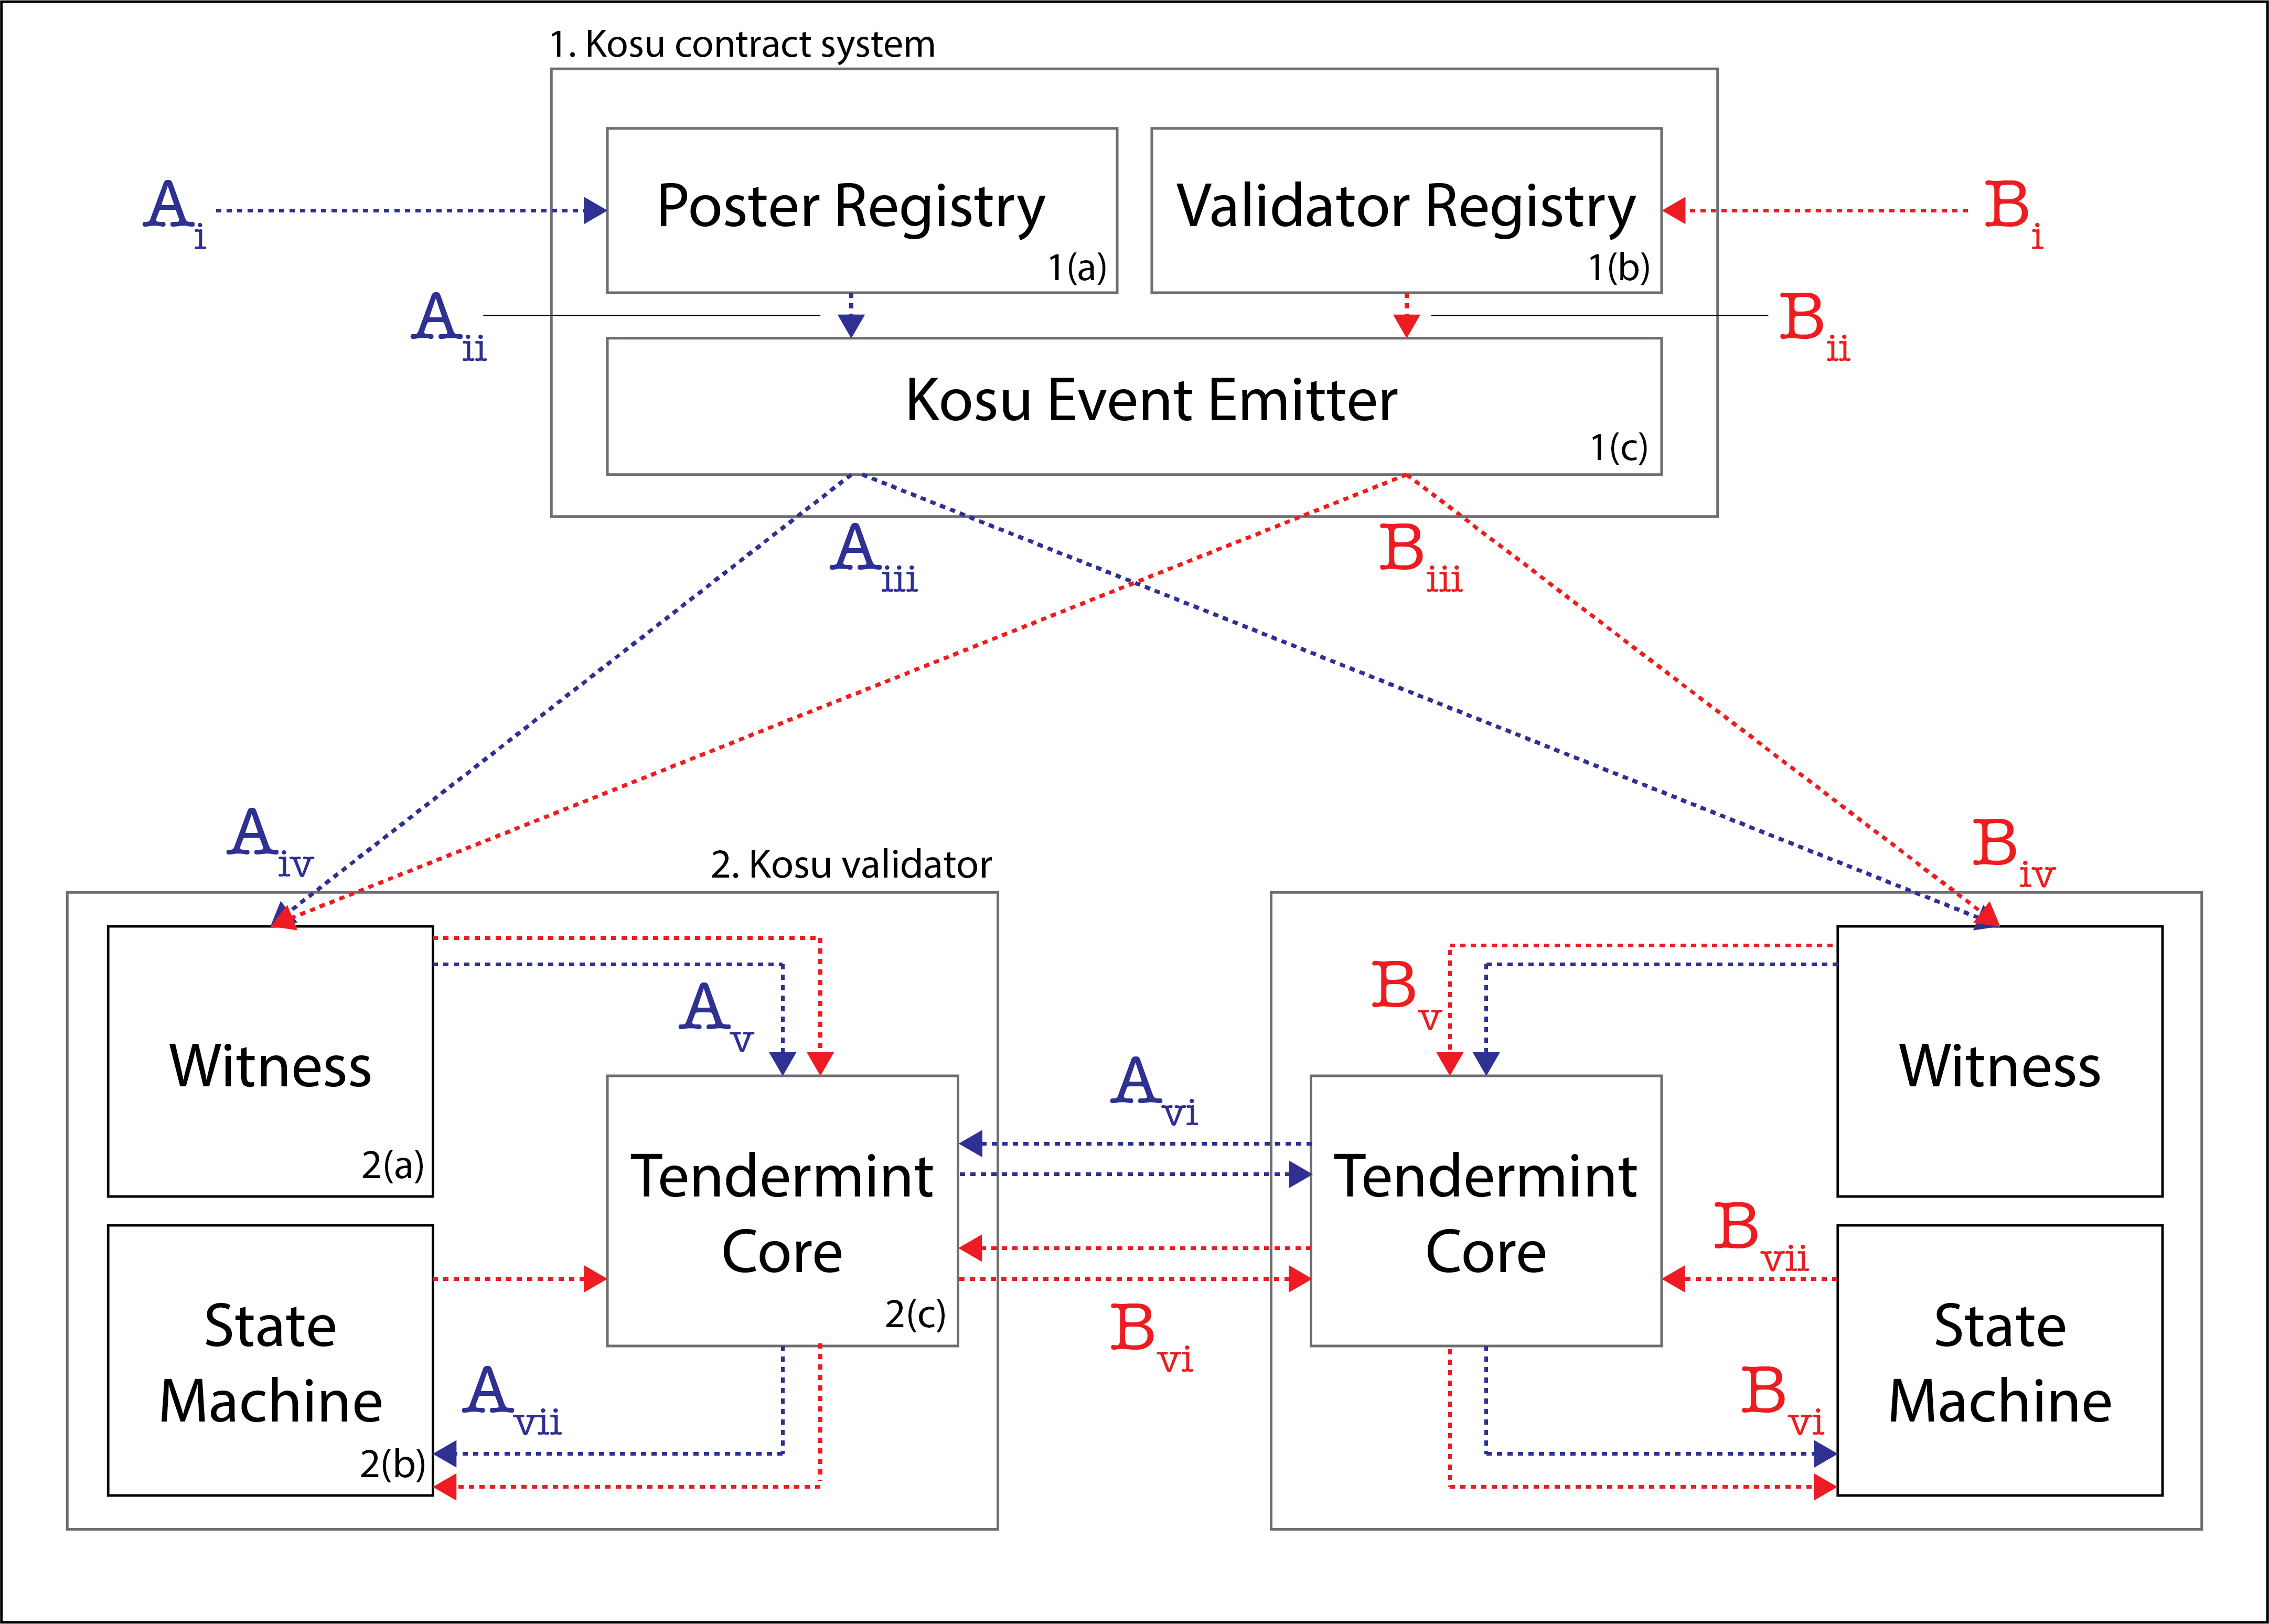
\includegraphics[width=\textwidth]{../figures/fig1.png}
  \caption{Simplified diagram of the systems involved in the Kosu-Ethereum peg zone. Box (1) shows components of the Kosu contract system, box (2) shows components of Kosu validators. The processes illustrated in red and blue are described below.}
  \label{fig:fig2}
\end{figure}
% END PEG SUB-SECTION
%%%%%%%%%%%%%%%%%%%%%%%%%%%%%%%%%%%%%%%%%%%%%%%%%%%%%%%%%%%%%%%%%%%%%%%%%%%%%%%%

%%%%%%%%%%%%%%%%%%%%%%%%%%%%%%%%%%%%%%%%%%%%%%%%%%%%%%%%%%%%%%%%%%%%%%%%%%%%%%%%
% BEGIN INCENTIVE MODEL SUB-SECTION
\subsection{Incentive Models}\label{incentive-models}

\subsubsection{Sybil tolerance}\label{incentive-models-sybil}
Poster bonding is the sybil tolerance mechanism used...=

\subsubsection{Validator elections}\label{incentive-models-val-elections}
During curation processes, voters can...

\subsubsection{Validator rewards}\label{incentive-models-val-rewards}
Validators can specify a reward in Kosu tokens... // cover burn case
% END INCENTIVE MODEL SUB-SECTION
%%%%%%%%%%%%%%%%%%%%%%%%%%%%%%%%%%%%%%%%%%%%%%%%%%%%%%%%%%%%%%%%%%%%%%%%%%%%%%%%

\clearpage
\pagebreak
% END SPECIFICATION SECTION

%%%%%%%%%%%%%%%%%%%%%%%%%%%%%%%%%%%%%%%%%%%%%%%%%%%%%%%%%%%%%%%%%%%%%%%%%%%%%%%%
%~~~~~~~~~~~~~~~~~~~~~~~~~~~~~~~~~~~~~~~~~~~~~~~~~~~~~~~~~~~~~~~~~~~~~~~~~~~~~~%
%%%%%%%%%%%%%%%%%%%%%%%%%%%%%%%%%%%%%%%%%%%%%%%%%%%%%%%%%%%%%%%%%%%%%%%%%%%%%%%%

% BEGIN TOKEN DISTRIBUTION SECTION
\section{Token Distribution}\label{token-distribution}

\subsection{Overview}\label{token-distribution-overview}
A continuous...

\subsection{Mechanics}\label{token-distribution-mechanics}
Such a model...

\subsection{Ether to Kosu}\label{token-distribution-eth-kosu}
ETH to KOSU...

\subsection{Kosu to Ether}\label{token-distribution-kosu-eth}
KOSU to ETH...\cite{bft}
\clearpage
\pagebreak
% END TOKEN DISTRIBUTION SECTION

%%%%%%%%%%%%%%%%%%%%%%%%%%%%%%%%%%%%%%%%%%%%%%%%%%%%%%%%%%%%%%%%%%%%%%%%%%%%%%%%
%~~~~~~~~~~~~~~~~~~~~~~~~~~~~~~~~~~~~~~~~~~~~~~~~~~~~~~~~~~~~~~~~~~~~~~~~~~~~~~%
%%%%%%%%%%%%%%%%%%%%%%%%%%%%%%%%%%%%%%%%%%%%%%%%%%%%%%%%%%%%%%%%%%%%%%%%%%%%%%%%

% BEGIN FUTURE WORK SECTION
\section{Future Work}\label{future-work}

\clearpage
\pagebreak
% END FUTURE WORK SECTION

%%%%%%%%%%%%%%%%%%%%%%%%%%%%%%%%%%%%%%%%%%%%%%%%%%%%%%%%%%%%%%%%%%%%%%%%%%%%%%%%
%~~~~~~~~~~~~~~~~~~~~~~~~~~~~~~~~~~~~~~~~~~~~~~~~~~~~~~~~~~~~~~~~~~~~~~~~~~~~~~%
%%%%%%%%%%%%%%%%%%%%%%%%%%%%%%%%%%%%%%%%%%%%%%%%%%%%%%%%%%%%%%%%%%%%%%%%%%%%%%%%

% BEGIN BIBLIOGRAPHY
\begin{thebibliography}{9}

\bibitem{peggy-spec}
Kunze, Federico, et al. "Two-way Permissionless Peg Zones." Tendermint.
\\\texttt{https://github.com/cosmos/peggy/tree/master/spec}

\bibitem{blockchain-taxonomy}
Tasca, Paola., Tessone, Claudio. J. "Taxonomy of Blockchain TechnologiesPrinciples of Identification and Classification."
\\\texttt{https://arxiv.org/pdf/1708.04872.pdf}

\bibitem{tendermint-wp}
Ethan Buchman, et al. "Tendermint: Byzantine Fault Tolerance in the Age of Blockchains."
\\\small\texttt{https://allquantor.at/blockchainbib/pdf/buchman2016tendermint.pdf}

\bibitem{0x-wp}
Warren, Will and Bandeali, Amir. "0x: An Open Protocol for Decentralized Exchange on the Ethereum Blockchain."
\\\texttt{https://github.com/0xProject/whitepaper/blob/master/0x\_white\_paper.pdf}

\bibitem{dharma-wp}
Hollander, Nadav. "Dharma: A Generic Protocol for Tokenized Debt Issuance."
\\\texttt{https://whitepaper.dharma.io}

\bibitem{tendermint}
All In Bits Inc., Tendermint, et al. "Tendermint Consensus Reactor."
\\\small\texttt{https://github.com/tendermint/tendermint/blob/master/docs/spec/reactors/consensus/consensus.md}

\bibitem{paradigm-github}
Paradigm Labs, corp., et al. "Paradigm Foundation GitHub."
\\\small\texttt{https://github.com/ParadigmFoundation/}

\bibitem{kosu-monorepo}
Paradigm Labs, corp., et al. "Kosu Monorepo: A Monorepo for the Kosu Protocol."
\\\small\texttt{https://github.com/ParadigmFoundation/kosu-monorepo}

\bibitem{kosu-sdk}
Freyaldenhoven, Nick., et al. "Kosu SubContract SDK."
\\\small\texttt{https://github.com/ParadigmFoundation/ParadigmContracts/blob/master/sdk/contracts/SubContract.sol}

\bibitem{bft}
Leslie Lamport, Robert Shostak, Marshall Pease. "The Byzantine Generals Problem."
\\ACM Transactions on Programming Languages and Systems, Vol. 4, No. 3. July 1982. Pages 382-401.

\end{thebibliography}

%%%%%%%%%%%%%%%%%%%%%%%%%%%%%%%%%%%%%%%%%%%%%%%%%%%%%%%%%%%%%%%%%%%%%%%%%%%%%%%%
%~~~~~~~~~~~~~~~~~~~~~~~~~~~~~~~~~~~~~~~~~~~~~~~~~~~~~~~~~~~~~~~~~~~~~~~~~~~~~~%
%%%%%%%%%%%%%%%%%%%%%%%%%%%%%%%%%%%%%%%%%%%%%%%%%%%%%%%%%%%%%%%%%%%%%%%%%%%%%%%%

% END BIBLIOGRAPHY
\end{document}
